% *****************************************************************
% Classic
% *****************************************************************
\usepackage[english]{babel}
\usepackage[utf8]{inputenc}
\usepackage[T1]{fontenc}
\usepackage{hyperref}


% ********** Basic supplementray materials
% \usepackage{hvfloat}  % rotation of caption
% \usepackage{rotating}  % allow complete rotation
\usepackage{soul}  % strikethrough text
\usepackage[normalem]{ulem}  % underline text
\usepackage{xcolor}  % color 
% **********


% ********** Maths packages
\usepackage{amssymb,amsmath}
\usepackage{graphicx}
% \usepackage{tikz}
% **********


% ********** Table packages
\usepackage{array}
\usepackage{booktabs}
\usepackage{colortbl}  % color cells
% \usepackage{longtable}
\usepackage{siunitx}
% \usepackage{tabu}
% \usepackage{threeparttable} 
% **********


% ********** Icones packages
\usepackage{fontawesome}
\usepackage{orcidlink}
\usepackage{tfrupee}
% **********


% ********** Define color + color configuration
\definecolor{NUred}{RGB}{213, 17, 45}
\definecolor{NUblue}{RGB}{0, 59, 113}
\definecolor{UBbrown}{RGB}{48, 33, 25}
\definecolor{UBblue}{RGB}{0, 158, 214}
\definecolor{ODRIISdarkgreen}{RGB}{80,151,68}
\definecolor{ODRIISlightgreen}{RGB}{164,204,76}
\definecolor{ODRIISbrick}{RGB}{197,102,63}
\definecolor{lightgray}{HTML}{A9A9A9}
\definecolor{lightgray2}{RGB}{113,113,113}
% **********
\hypersetup{colorlinks,linkcolor={lightgray2},citecolor={ODRIISdarkgreen},urlcolor={ODRIISdarkgreen}}
%\renewcommand{\beamertextcolor}{}
%\renewcommand{\beamerbgcolor}{}
%\renewcommand{\beamerfootertextcolor}{}
\renewcommand{\beamertitlecolor}{ODRIISbrick}
\setbeamercolor{button}{bg=ODRIISdarkgreen,fg=ODRIISlightgreen!10}
% **********





% *****************************************************************
% Pureminimalistic configuration
% *****************************************************************
\renewcommand{\logotitle}{\vspace*{-20mm}\hspace*{-10.1mm}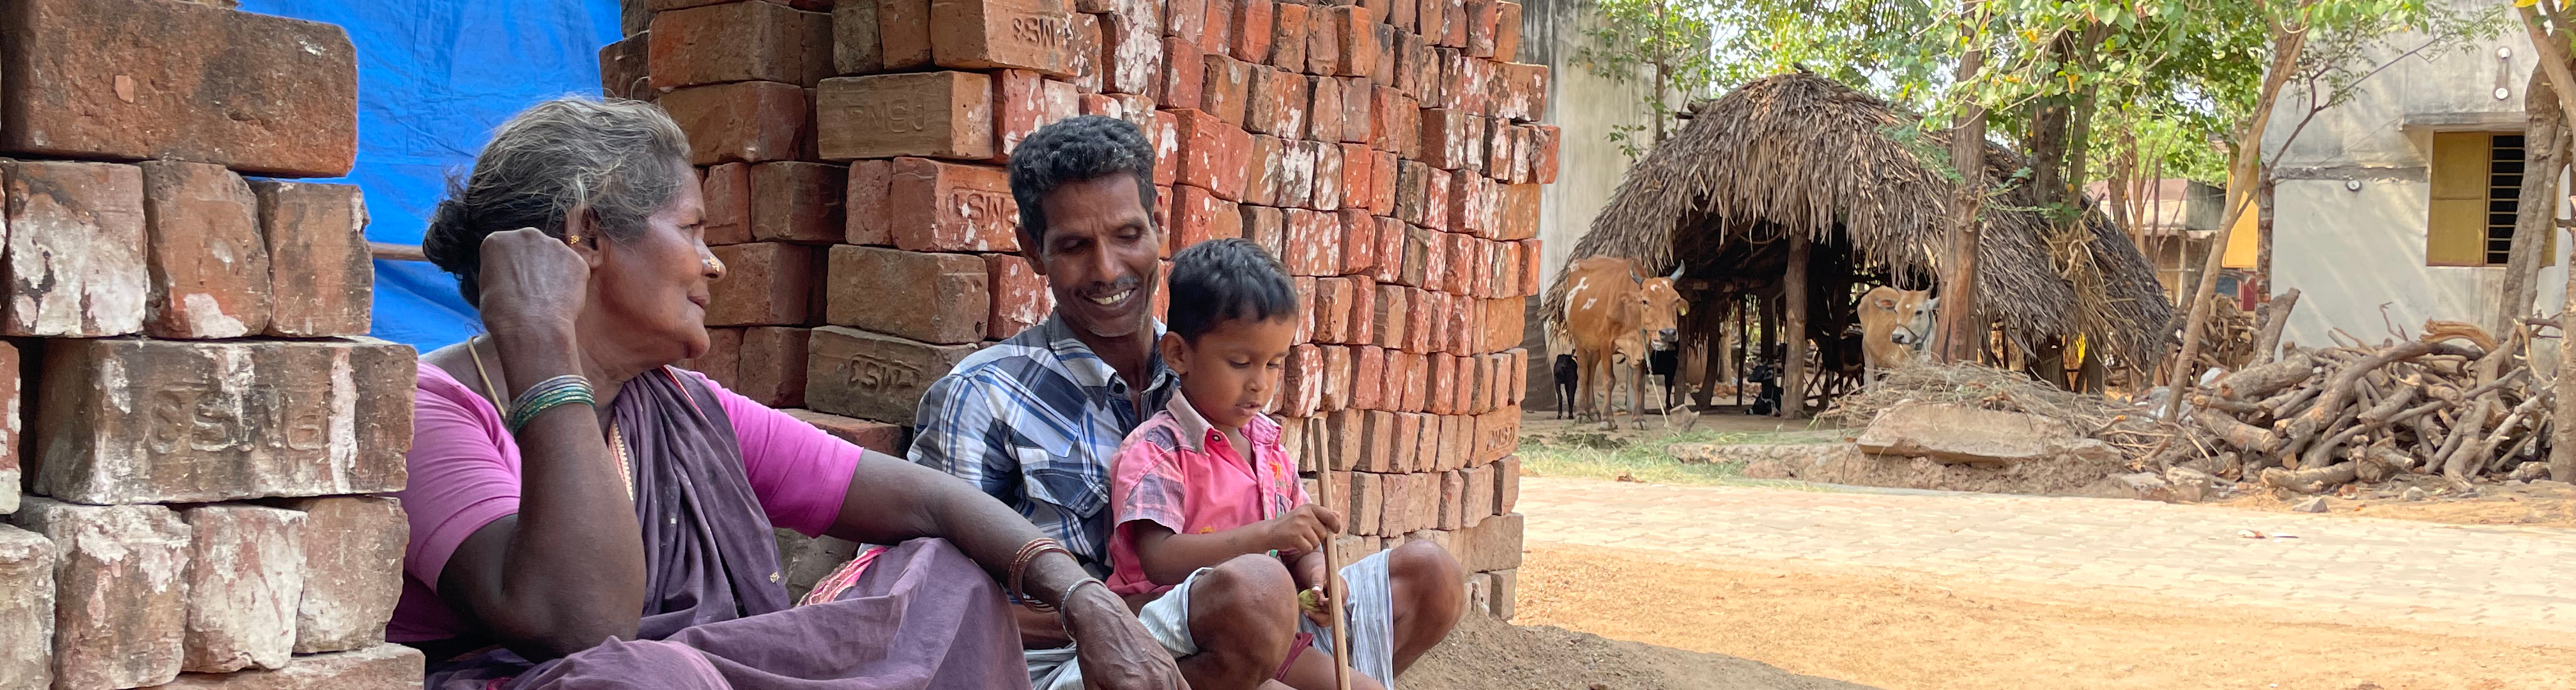
\includegraphics[width=\paperwidth]{Beamer_theme/header.jpeg}}
\renewcommand{\logoheader}{\vspace{0em}}
\renewcommand{\logoheader}{\vspace{0em}}
\renewcommand{\logofooter}{\href{https://odriis.hypotheses.org/}{
\includegraphics[width=.6\linewidth]{Beamer_theme/odriis_long.png}}}



% *****************************************************************
% Caption configuration
% *****************************************************************
\usepackage{caption}  % custom caption

\captionsetup{
font=small,
skip=1em,
labelfont={bf},
justification=centering,
singlelinecheck=false,
%textfont={bf,it},
%labelsep=endash,
%tableposition=top,
}






% *****************************************************************
% Appendix
% *****************************************************************
\usepackage{appendixnumberbeamer}
\renewcommand{\appendixname}{\texorpdfstring{\translate{appendix}}{appendix}}





% *****************************************************************
% Bibliography
% *****************************************************************

% ********** Bibtex
% \usepackage[doi, natbibapa]{apacite}
% \renewcommand\bibliographytypesize{\tiny}
% \let\realcitep\citep
% \renewcommand*{\citep}[1]{{\small\realcitep{#1}}}
% \let\realcite\cite
% \renewcommand*{\cite}[1]{{\small\realcite{#1}}}
% ********** 


% ********** Biblatex
\usepackage[
natbib=true,
backend=biber,
style=trad-abbrv,
sorting=none, %nyt
]{biblatex}
% **********
\renewcommand*{\bibfont}{\footnotesize}





% *****************************************************************
% Bigcenter
% *****************************************************************
\makeatletter
\newskip\@bigflushglue \@bigflushglue = -100pt plus 1fil
\def\bigcenter{\trivlist \bigcentering\item\relax}
\def\bigcentering{\let\\\@centercr\rightskip\@bigflushglue%
\leftskip\@bigflushglue
\parindent\z@\parfillskip\z@skip}
\def\endbigcenter{\endtrivlist}
\makeatother






% *****************************************************************
% Box creation
% *****************************************************************
\usepackage[most]{tcolorbox}

\newtcolorbox{greenbox}[2][]{colback=ODRIISlightgreen!10,colframe=ODRIISlightgreen!10,coltitle=black,colbacktitle=ODRIISdarkgreen!20,title={#2},#1}
\newtcolorbox{brickbox}[1][]{colback=ODRIISbrick!10,colframe=ODRIISbrick!10,#1}






% *****************************************************************
% Section page
% *****************************************************************
\newcommand{\secttitle}[1]{
\begin{columns} 
\begin{column}{.4\textwidth}
\vspace*{-0mm}\hspace*{-10.1mm}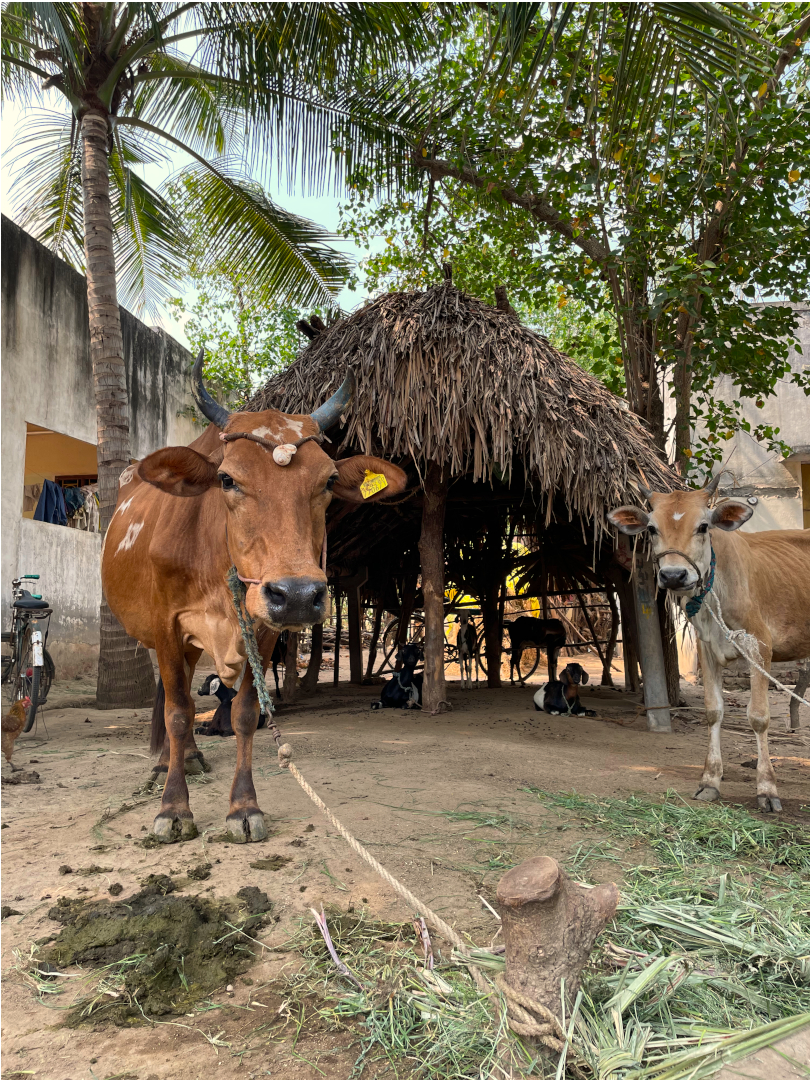
\includegraphics[height=\paperheight]{Beamer_theme/cow.jpeg}
\end{column}
\begin{column}{.6\textwidth}
\vfill
\begin{tcolorbox}[colback=ODRIISlightgreen!20,colframe=ODRIISlightgreen!20,box align=center,halign=center,valign=center]
{\LARGE \textcolor{ODRIISbrick}{#1}}
\end{tcolorbox}
\vfill
\end{column}
\end{columns}
}






% *****************************************************************
% Table
% *****************************************************************

% ********** Stars
\newcommand{\sym}[1]{\rlap{#1}}% Thanks to David Carlisle
% **********


% ********** Insert the table
\newcommand{\inserttable}[3]{
\resizebox{#3}{!}{
\begin{tabular}{#2}
\toprule
\input #1
\bottomrule
\end{tabular}
}
}
% **********


% ********** Source
\newcommand{\bottomtext}[1]{\vspace{-1.5ex}\captionsetup{justification=centering,font=footnotesize,singlelinecheck=false}\caption*{\hangindent=1.5em #1}}
\newcommand{\bottomnote}[1]{\bottomtext{\textit{Note}:~#1}}
\newcommand{\source}[1]{\bottomtext{\textit{Source}:~#1}}
\newcommand{\starnote}{\bottomtext{* p < 0.1, ** p < 0.05, *** p < 0.01. Standard error in parentheses.}}
% **********


% ********** siunitx config
\sisetup{
detect-mode,
tight-spacing= true,
group-digits= false ,
input-signs= ,
input-symbols= ( ) [ ] - + *,
input-open-uncertainty=,
input-close-uncertainty=,
table-align-text-post=false
}
% **********


% ********** Linebreak in cell
\newcommand{\specialcell}[2][c]{\begin{tabular}[#1]{@{}c@{}}#2\end{tabular}}
% **********


% \makeatletter
% \AddToHook{env/tabular/begin}{\let\input\@@input}
% \makeatother




% *****************************************************************
% Personnal cmd
% *****************************************************************
\newcommand{\jati}[1]{\textit{j\={a}ti{#1}}}

\newcommand\dev[1]{\textbf{\textcolor{red}{#1}}}

\newcommand{\ie}{i.e.}
\newcommand{\sd}{standard deviation}
\newcommand{\pp}{percentage points}
\newcommand{\aebe}{all else being equal}
\newcommand{\Aebe}{All else being equal}
\newcommand{\ote}{other things equal}
\newcommand{\Ote}{Other things equal}
\newcommand{\cl}{confidence level}
\newcommand{\lit}{\dev{literature}}
\newcommand{\PTCS}{PT\&CS}

\newcommand{\key}[1]{\underline{\textsc{#1}}}
\newcommand{\data}[1]{\textbf{\underline{Data #1:}}~}


% ********** Symbol shortcuts
\def\@fnsymbol#1{\ensuremath{\ifcase#1\or *\or \dagger\or \ddagger\or
   \mathsection\or \mathparagraph\or \|\or **\or \dagger\dagger
   \or \ddagger\ddagger \else\@ctrerr\fi}}
   
\makeatletter
\newcommand{\ssymbol}[1]{^{\@fnsymbol{#1}}}
\makeatother
% **********